\documentclass[10pt,landscape]{article}
\usepackage{multicol}
\usepackage{amsfonts}
\usepackage{calc}
\usepackage{ifthen}
\usepackage[landscape]{geometry}
\usepackage{hyperref}
\usepackage{stmaryrd}
\usepackage{amsmath}
\usepackage{tikz}

\usepackage[utf8]{inputenc}
\usepackage[T1]{fontenc}

\DeclareMathOperator*{\argmax}{arg\,max}


% This sets page margins to .5 inch if using letter paper, and to 1cm
% if using A4 paper. (This probably isn't strictly necessary.)
% If using another size paper, use default 1cm margins.
\ifthenelse{\lengthtest { \paperwidth = 11in}}
	{ \geometry{top=.5in,left=.5in,right=.5in,bottom=.5in} }
	{\ifthenelse{ \lengthtest{ \paperwidth = 297mm}}
		{\geometry{top=1cm,left=1cm,right=1cm,bottom=1cm} }
		{\geometry{top=1cm,left=1cm,right=1cm,bottom=1cm} }
	}

% Turn off header and footer
\pagestyle{empty}
 

% Redefine section commands to use less space
\makeatletter
\renewcommand{\section}{\@startsection{section}{1}{0mm}%
                                {-1ex plus -.5ex minus -.2ex}%
                                {0.5ex plus .2ex}%x
                                {\normalfont\large\bfseries}}
\renewcommand{\subsection}{\@startsection{subsection}{2}{0mm}%
                                {-1explus -.5ex minus -.2ex}%
                                {0.5ex plus .2ex}%
                                {\normalfont\normalsize\bfseries}}
\renewcommand{\subsubsection}{\@startsection{subsubsection}{3}{0mm}%
                                {-1ex plus -.5ex minus -.2ex}%
                                {1ex plus .2ex}%
                                {\normalfont\small\bfseries}}
\makeatother

% Define BibTeX command
\def\BibTeX{{\rm B\kern-.05em{\sc i\kern-.025em b}\kern-.08em
    T\kern-.1667em\lower.7ex\hbox{E}\kern-.125emX}}

% Don't print section numbers
\setcounter{secnumdepth}{0}


\setlength{\parindent}{0pt}
\setlength{\parskip}{0pt plus 0.5ex}


% -----------------------------------------------------------------------

\begin{document}

\raggedright
\footnotesize
\begin{multicols}{3}


% multicol parameters
% These lengths are set only within the two main columns
%\setlength{\columnseprule}{0.25pt}
\setlength{\premulticols}{1pt}
\setlength{\postmulticols}{1pt}
\setlength{\multicolsep}{1pt}
\setlength{\columnsep}{2pt}

\begin{center}
     \Large{\textbf{IFT6266 Cheat Sheet}} \\
     Thomas George 2016
\end{center}

\section{Machine learning basics}

\subsection{Some distributions}

\begin{itemize}
\item \textbf{Bernoulli} : $P(x=1) = \phi$, $P(x=0) = 1 - \phi$
\item \textbf{Gaussian} : $\mathcal{N}(x; \mu, \sigma^2) = \sqrt{\frac{1}{2 \pi \sigma^2}} \exp \Big( - \frac{1}{2 \sigma^2} (x - \mu)^2 \Big)$
\item \textbf{Laplace} : $\text{Laplace}(x; \mu, \gamma) = \frac{1}{2 \gamma} \exp \Big( - \frac{\lvert x - \mu \rvert}{\gamma} \Big)$
\end{itemize}

\subsection{Entropy}

$$H(P) = \mathbb{E}_{x \sim P}[- \log P(x)]$$

\subsection{Cross-entropy}

$$H(P,Q) = \mathbb{E}_{x \sim P}[- \log Q(x)]$$

\subsection{Kullback-Leibler divergence}

$$D_{KL}(P \lVert Q) = \mathbb{E}_{x \sim P}\Big[\log \frac{P(x)}{Q(x)} \Big]$$

\subsection{Maximum likelihood estimator}

$$\mathbf{\theta}_{ML} = \argmax_\theta p_{\text{model}}(\mathbb{X}; \theta) = \argmax_\theta \prod_{i=1}^m p_{\text{model}}(\mathbf{x}^{(i)}; \theta)$$
where the $x_i$s are samples from the empirical distribution $\hat p_\text{data}$. Same but expressed in term of log and rescaled by $\frac{1}{m}$:

$$\mathbf{\theta}_{ML} = \argmax_\theta \mathbb{E}_{\mathbf{x} \sim \hat p_\text{data}} \big[ \log p_{\text{model}}(\mathbf{x}; \mathbf{\theta}) \big]$$

can be derived by minimizing $D_{KL}(\hat{p}_\text{data} \lVert p_\text{model})$ for the empirical dataset.

\subsection{Bias, variance, MSE}

$$\text{Bias}(\hat \theta_m) = \mathbb{E}(\hat \theta_m) - \theta$$
$$\text{Var}(\hat \theta_m)$$
$$\text{MSE}(\hat \theta_m) = \text{Bias}(\hat \theta_m)^2 + \text{Var}(\hat \theta_m)$$

\section{Neural networks basics}

\subsection{Multilayer perceptron}

\subsection{Convolutional networks}

\subsection{Recurrent networks}

\subsection{Activation functions}

\begin{itemize}
\item \textbf{Logistic sigmoid} : $\sigma(\mathbf x) = \frac{1}{1+\exp(- \mathbf x)}$
\item \textbf{Softplus} : $\zeta(\mathbf x) = \log(1 + \exp(\mathbf x))$
\item \textbf{Rectifier} : $\text{ReLU}(\mathbf x) = \max(0,\mathbf x)$
\item \textbf{Leaky ReLU} : $\text{Leaky}(\mathbf x) = \max(a \mathbf x, \mathbf x)$ ($a \in [0,1]$)
\item \textbf{Softmax} : $\text{softmax}(\mathbf{x})_i = \frac{\exp(x_i)}{\sum_j \exp(x_j)}$
\end{itemize}

\section{Regularization}

\subsection{L1}

Results in a solution that is more sparse.

\subsection{L2}

The regularizer has a strong effect along axis where the objective function does not change much. It is equivalent to MAP bayesian inference with a Gaussian prior on the weights.

\subsection{Early stopping}

Equivalent to L2 for a simple linear model with quadratic error.

\subsection{Sparsity regularization}

Add term $\Omega(h)$ to the cost where $h$ is a hidden representation.

\subsection{Data augmentation}

\subsection{Dropout}

\section{Optimization}

\subsection{Jacobian matrix}

$$J_{i,j} = \frac{\partial}{\partial x_j} f(\mathbf{x})_i$$

\subsection{Hessian matrix}

$$\mathbf{H}(f)(\mathbf{x})_{i,j} = \frac{\partial^2}{\partial x_i\partial x_j} f(\mathbf{x})$$

\subsection{Newton's method}

$$\mathbf{x}^* = \mathbf{x}^{(0)} - \mathbf{H}(f)(\mathbf{x}^{(0)})^{-1} \nabla_x f(\mathbf{x}^{(0)})$$

\subsection{Backpropagation}

\subsection{Stochastic gradient descent}

\section{Autoencoders}

Encoder $f$, decoder $g$:
$$\mathcal{J}_{AE}(\theta) = \sum_x L(x, g(f(x)))$$ where the reconstruction error $L$ can be the squared error for linear reconstruction or maximum likelihood for sigmoid outputs.

\subsection{Regularized autoencoders}

Add weigth decay over the parameters.

\subsection{Denoising autoencoders}

Corrupt $x$ before sending it through the auto-encoder:
$$\mathcal{J}_{DAE}(\theta) = \sum_x \mathbb{E}_{\tilde x \sim q(\tilde x \lvert x)} \big[ L(x, g(f(\tilde x))) \big]$$

\subsection{Contractive autoencoders}

Add a regularization over the Foebius norm of the Jacobian :

$$\lVert J_f(x) \rVert_F^2 = \sum_{ij} \Big( \frac{\partial h_j(x)}{\partial x_i} \Big)^2$$

\section{Representation learning}

\section{Graphical models}

\subsection{Basics}

\subsubsection{Directed graphical models}

$$p(\mathbf{x}) = \prod_i p(x_i \lvert Pa_{\mathcal{G}}(x_i))$$

\subsubsection{Undirected graphical models}

$$p(\mathbf{x}) = \frac{1}{Z} \prod_i \phi^{(i)} \Big( \mathcal{C}^{(i)} \Big)$$

over the cliques $\mathcal{C}^{(i)}$. 

\subsection{Restricted Boltzmann machines}

\begin{center}
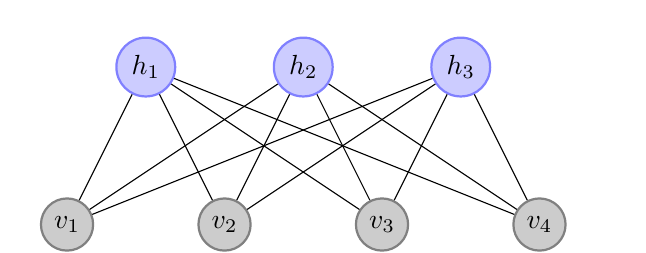
\begin{tikzpicture}
  [inner sep=1mm,
   hidden/.style={circle,draw=blue!50,fill=blue!20,thick},
   visible/.style={circle,draw=black!50,fill=black!20,thick}]
  \useasboundingbox (-0.5,0) rectangle (7,2.5);
  \node at (0,0) (v1) [visible] {$v_1$};
  \node at (2,0) (v2) [visible] {$v_2$};
  \node at (4,0) (v3) [visible] {$v_3$};
  \node at (6,0) (v4) [visible] {$v_4$};
  \node at (1,2) (h1) [hidden] {$h_1$};
  \node at (3,2) (h2) [hidden] {$h_2$};
  \node at (5,2) (h3) [hidden] {$h_3$};
  \foreach \x in {1,...,4}
     \foreach \y in {1,...,3}
       \draw [-] (v\x) to (h\y);
\end{tikzpicture}
\end{center}

$$E(\mathbf v,\mathbf h)=-\mathbf{b}^T \mathbf{v} - \mathbf c^T \mathbf h - \mathbf v^T \mathbf W \mathbf h$$
$$p(\mathbf v,\mathbf h)=\frac{1}{Z}e^{-E(\mathbf v,\mathbf h)}$$
\begin{center}
$p(\mathbf v \lvert \mathbf h) = \prod_i p(v_i \lvert \mathbf{h})$ and $p(\mathbf h \lvert \mathbf v) = \prod_i p(h_i \lvert \mathbf{v})$
$$p(h_i = 1 \lvert \mathbf v) = \sigma \big( \mathbf v^T \mathbf W_{:,i} + b_i \big)$$
\end{center}
The intractable $p(\mathbf{v}) = \sum_{\mathbf{h}} p(\mathbf{v}, \mathbf{h})$ can be rewritten:
$$p(\mathbf{v}) = \frac{1}{Z} \exp \Big( \mathbf{b}^T \mathbf{v} + \sum_{j=1}^H \text{softplus} \big(c_j + \mathbf{v}^T \mathbf{W}_.j \big) \Big)$$
\subsection{Deep Belief Networks}

\subsection{Deep Boltzmann Machines}

\subsection{Variational Auto Encoders}

\subsection{Generative Adversarial Networks}

\section{Partition function}

Log-likelihood for an undirected model $p(\mathbf x;\mathbf \theta) = \frac{1}{Z(\mathbf{\theta})} \tilde p(\mathbf x;\mathbf \theta)$:
$$\nabla_{\theta} \log p(\mathbf x;\mathbf \theta) = \nabla_{\theta} \log \tilde p(\mathbf x;\mathbf \theta) - \nabla_{\theta} \log Z(\mathbf \theta)$$

The first term is called the positive phase, the second term the negative phase and we have:

$$\nabla_{\theta} \log Z(\mathbf \theta) = \mathbb{E}_{\mathbf{x} \sim p(\mathbf{x})} \nabla_{\theta} \log \tilde p(\mathbf x)$$

\subsection{Stochastic maximum likelihood algorithm}

The method to get an estimate of the gradient to do a gradient descent step is:
\begin{enumerate}
\item Sample a minibatch of $m$ examples from the training set
\item $\mathbf g \leftarrow \frac{1}{m} \sum_{i=1}^m \nabla_{\theta} \log \tilde p(\mathbf x^{(i)};\mathbf \theta)$
\item Initialize a set of $m$ samples to random values
\item for all samples, do $k$ Gibbs steps, high enough to burn in, to get a good sample from $\tilde p$.
\item $\mathbf g \leftarrow \mathbf g - \frac{1}{m} \sum_{i=1}^m \nabla_{\theta} \log \tilde p(\tilde{\mathbf{x}}^{(i)};\mathbf \theta)$
\end{enumerate}

\subsection{Contrastive divergence}

Same as above, but start from examples from the training set instead of random samples for the negative phase. We do not require the many Gibbs steps needed for burn in (1 might be enough).

It fails at suppressing \textbf{spurious modes}, modes that have high probability under the model but low probability under the data generating distribution.

\subsection{Persistent contrastive divergence}

Start the sampling step from the previous samples. It is more resistant to forming models with spurious than CD.

Also provides starting points for sampling for both visible and hidden units (as opposite to visible only for CD).


\section{Sampling methods}

\subsection{Monte-Carlo}

$$\hat s_n = \frac{1}{n} \sum_{i=1, \mathbf{x}^{(i)} \sim p}^n f(\mathbf{x}^{(i)})$$

\subsection{MCMC}

TODO
 
Problem: it mixes poorly between modes. This can be attenuated by adding a temperature parameter $p_{\beta} (\mathbf{x}) \propto \exp(-\beta E(\mathbf{x}))$.

\subsection{Ancestral sampling}

For directed graphical models, using the topological ordering, draw sequentially samples from $p(x_i \lvert Pa_{\mathcal{G}}(x_i))$

\subsection{Gibbs sampling}

For undirected graphical models, draw samples from $p(x_i \lvert x_{-i})$. Asymptotically, it converges to sampling from the correct distribution.

Block Gibbs sampling can be used i.e. in RBMs where we have a closed form for $p(\mathbf v \lvert \mathbf h)$ and $p(\mathbf h \lvert \mathbf v)$.

\subsection{Importance sampling}

$$\hat s_q = \frac{1}{n} \sum_{i=1, \mathbf{x}^{(i)} \sim q}^n \frac{p(\mathbf{x}^{(i)}) f(\mathbf{x}^{(i)})}{q(\mathbf{x}^{(i)})}$$

\section{Approximate inference}

\textbf{Inference}: computing $p(\mathbf{h} \lvert \mathbf{v})$ or its expectation.

\subsection{Variational free energy}

Also called \textbf{evidence lower bound}:

$$\mathcal{L}(\mathbf{v}; \mathbf{\theta}, q) = \log p(\mathbf{v}, \mathbf{\theta}) - D_{KL} \big( q(\mathbf{h} \lvert \mathbf{v}) \lVert p(\mathbf{h} \lvert \mathbf{v}; \mathbf{\theta}) \big)$$ (as opposed to maximum likelihood where we minimize $D_{KL}(\hat{p}_\text{data} \lVert p_\text{model})$)

A more canonical definition is:

$$\mathcal{L}(\mathbf{v}; \mathbf{\theta}, q) = \mathbb{E}_{\mathbf h \sim q} [ \log p(\mathbf h, \mathbf v)] + H(q)$$

\subsection{Expectation maximization}

\begin{itemize}
\item \textit{E-step}: Maximize $\mathcal{L}$ w.r.t. $q$ i.e. find $q$ that best approximates $p$ on the training dataset
\item \textit{M-step}: Maximize $\mathcal{L}$ w.r.t. $\theta$
\end{itemize}

\subsection{MAP inference}
Find the single most likely value using \textit{maximum a posteriori} inference:

$$\mathbf{h}^* = \argmax_{\mathbf{h}} p(\mathbf{h} \lvert \mathbf{v})$$


\end{multicols}
\end{document}
